\section{Alternative approaches to the proposed empirical Bernstein inequality} \label{section:alternative_approaches}

We present in this appendix two alternative approaches to that proposed in Section~\ref{section:main_results}. 


\subsection{Decoupling the inequality into first and second moment inequalities} \label{section:naive_approach_two_eb}

We start by presenting a naive approach to the problem using two empirical Bernstein inequalities, which may be the most natural starting point. However, this approach will prove suboptimal, both theoretically and empirically.


\subsubsection{Confidence sequences obtained using two empirical Bernstein inequalities} 
We start by noting that
\begin{align*}
    \sigma^2 = \E X_i^2 - \E^2X_i,
\end{align*}
Thus, in order to give an upper confidence sequence for $\sigma^2$, it suffices to derive an upper confidence sequence for $\E X_i^2$ and a lower confidence sequence for $\E X_i$. Consider
\begin{align*}
    U_{1, \alpha_1, t} :=  \frac{\sum_{i \leq t}\lambda_i (X_i^2 - \widehat {m_2}_i)^2}{\sum_{i \leq t} \lambda_i} + \frac{\log(1/\alpha_1) + \sum_{i \leq t}\psi_E(\lambda_i) \lp X_i ^2 - \widehat {m_2}_i \rp^2}{\sum_{i \leq t} \lambda_i} 
\end{align*}
as the upper confidence sequence for $\E X_i^2$ (which follows from empirical Bernstein inequality), and 
\begin{align*}
    L_{2, \alpha_2, t} :=   \frac{\sum_{i \leq t} \tilde \lambda_i X_i}{\sum_{i \leq t} \tilde \lambda_i} - \frac{\log(1/\alpha_1) + \sum_{i \leq t}\psi_E(\tilde\lambda_i) \lp X_i - \widehat \mu_i \rp^2}{\sum_{i \leq t} \tilde \lambda_i} 
\end{align*}
as the lower confidence sequence for $\E X_i$ (which follows from empirical Bernstein), so that $\alpha_1 + \alpha_2 = \alpha$. Now we take
\begin{align}
    \sigma^2 \leq U_{1, \alpha_1, t} - L^2_{2, \alpha_2, t}
\end{align}
as the upper confidence sequence for $\sigma^2$.

Similarly, in order to derive lower inequalities, define
\begin{align*}
    L_{1, \alpha_1, t} :=  \frac{\sum_{i \leq t}\lambda_i (X_i^2 - \widehat {m_2}_i)^2}{\sum_{i \leq t} \lambda_i} - \frac{\log(1/\alpha_1) + \sum_{i \leq t}\psi_E(\lambda_i) \lp X_i ^2 - \widehat {m_2}_i \rp^2}{\sum_{i \leq t} \lambda_i} 
\end{align*}
as the lower confidence sequence for $\E X_i^2$ (which follows from empirical Bernstein inequality), and 
\begin{align*}
    L_{2, \alpha_2, t} :=   \frac{\sum_{i \leq t} \tilde \lambda_i X_i}{\sum_{i \leq t} \tilde \lambda_i} + \frac{\log(1/\alpha_1) + \sum_{i \leq t}\psi_E(\tilde\lambda_i) \lp X_i - \widehat \mu_i \rp^2}{\sum_{i \leq t} \tilde \lambda_i} 
\end{align*}
as the upper confidence sequence for $\E X_i$ (which follows from empirical Bernstein), so that $\alpha_1 + \alpha_2 = \alpha$. Now we take
\begin{align}
    \sigma^2 \geq L_{1, \alpha_1, t} - U^2_{2, \alpha_2, t}
\end{align}
as the lower confidence sequence for $\sigma^2$. 



\subsubsection{Theoretical and empirical suboptimality of the approach}

Ideally, we would expect the width of the confidence interval for $\sigma^2$ to scale as $ \sqrt{2\V (X-\mu)^2\log(1/\alpha)/t}$ (i.e., first order term in Bennett's inequality). However, we see that the term in $U_{1, \alpha_1, t}$
\begin{align*}
     \frac{\log(1/\alpha_1) + \sum_{i \leq t}\psi_E(\lambda_i) \lp X_i ^2 - \widehat {m_2}_i \rp^2}{\sum_{i \leq t} \lambda_i}
\end{align*}
scales as $ \sqrt{2\V X^2\log(1/\alpha)/t}$. It suffices to observe that
\begin{align*}
    \V (X-\mu)^2 &= \E (X-\mu)^4 - \E^2 (X-\mu)^2
    \\&= \E \lb X^4 - 4X^3\mu + 6X^2\mu^2 - 4X\mu^3 + \mu^4 \rb - \lb \E^2X^2 + \mu^4 - 2 \mu^2\E X^2  \rb
    \\&=\lp  \E X^4 - \E^2 X^2 \rp + \E \lb - 4X^3\mu + 8X^2\mu^2 - 4X\mu^3  \rb
    \\&= \lp  \E X^4 - \E^2 X^2 \rp - 4\mu \E \lp X^{\frac{3}{2}} - X^{\frac{1}{2}}\mu \rp^2
    \\&= \V X^2 - 4\mu \E \lp X^{\frac{3}{2}} - X^{\frac{1}{2}}\mu \rp^2
    \\&\leq \V X^2,
\end{align*}
where the last inequality follows from $\mu \in (0,1)$, to conclude that the first order term of this confidence interval will generally dominate that of Bennett's inequality.

We also clearly see the suboptimality of the approach empirically.  Figure~\ref{fig:eb_vs_decoupled} exhibits the upper and lower inequalities proposed in Section~\ref{section:main_results} to those derived in this appendix for all the scenarios considered in Section~\ref{section:experiments}, illustrating the poor performance of the latter.

\begin{figure}[ht] 
    \center 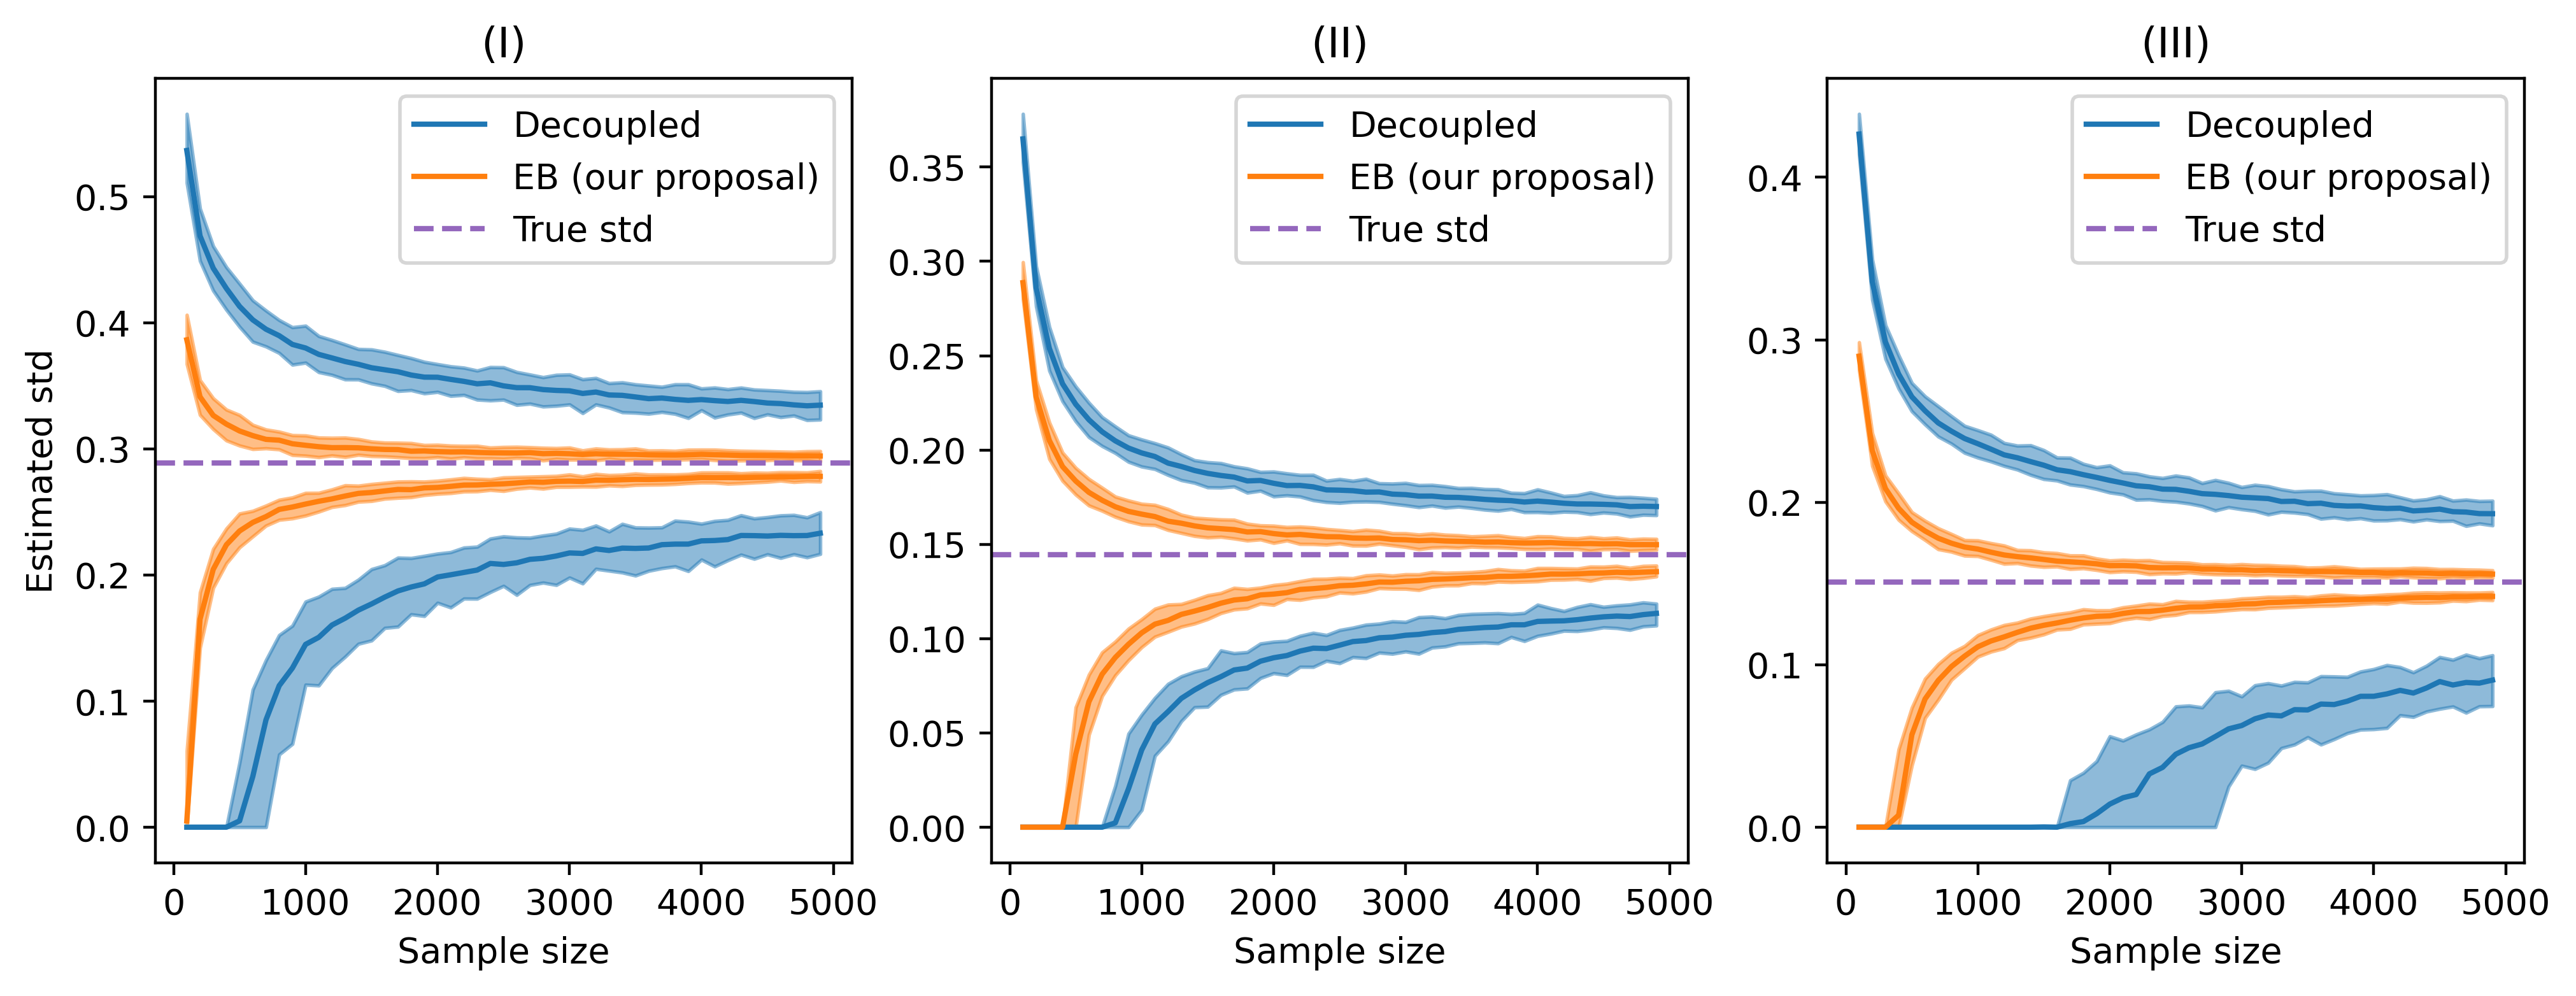
\includegraphics[width=\textwidth]{plots/eb_vs_decoupled.png}
  \caption{Average confidence intervals over $100$ simulations for the std $\sigma$ for (I) the uniform distribution in $(0,1)$, (II) the beta distribution with parameters $(2, 6)$, and (III) the beta distribution with parameters $(5, 5)$. For each of the inequalities, the $0.95\%$-empirical quantiles are also displayed. The decoupling approach (this appendix) is compared against EB (our proposal). EB clearly outperforms the decoupled approach in all the scenarios.} 
  \label{fig:eb_vs_decoupled}
\end{figure}


\subsection{Upper bounding the error term instead of taking negligible plug-ins}

In Section~\ref{section:lower_bound}, we proposed to take $\lambda_{t, l ,\alpha_2} = 0$ if
\begin{align*}
    \frac{\log(2/\alpha_1) + \hat\sigma^2_{t} \sum_{i=1}^{t-1} \psi_P(\tilde \lambda_i)}{\sum_{i=1}^{t-1} \tilde \lambda_i} \leq 1.
\end{align*}
A reasonable alternative would be to avoid defining $\lambda_{t, l ,\alpha_2}$ as $0$ (i.e., always define $\lambda_{t, l ,\alpha_2} := \lambda_{t, u ,\alpha_2}$), and to take
\begin{align*}
    \tilde R_{t, \delta} = \begin{cases}
        \frac{\log(2/\delta) + \sigma^2\sum_{i=1}^{t-1} \psi_P(\tilde \lambda_i)}{\sum_{i=1}^{t-1} \tilde \lambda_i}, \quad &\text{if} \quad \frac{\log(2/\delta) + \hat\sigma^2_{t-1} \sum_{i=1}^{t-1} \psi_P(\tilde \lambda_i)}{\sum_{i=1}^{t-1} \tilde \lambda_i} \leq 1, \\
        1, \quad &\text{otherwise}.
    \end{cases}
\end{align*}
In order to formalize this, denote
\begin{align*}
    \Upsilon_t := \lc i \in [t] : \frac{\log(2/\delta) + \hat\sigma^2_{t-1}\sum_{i=1}^{t-1} \psi_P(\tilde \lambda_i)}{\sum_{i=1}^{t-1} \tilde \lambda_i} \leq 1 \rc, \quad  \Upsilon_t^c := [t] \backslash \Upsilon_t.
\end{align*}
Taking
\begin{align*}
    A_{t} &:=  \frac{\sum_{i \in \Upsilon_t}\lambda_i \tilde A_{i}}{\sum_{i \leq t} \lambda_i}, 
    \quad B_{t, \delta} := 1 +  \frac{\sum_{i \in \Upsilon_t}\lambda_i \tilde B_{i, \delta}}{\sum_{i \leq t} \lambda_i},
    \\ C_{t, \delta} &:= \frac{\sum_{i \in \Upsilon_t}\lambda_i \tilde C_{i, \delta} + \sum_{i \in \Upsilon_t^c}\lambda_i}{\sum_{i \leq t} \lambda_i},
\end{align*}
in Section~\ref{section:lower_bound}, Corollary~\ref{corollary:lower_bound} also holds. Figure~\ref{fig:eb_vs_ebalternative} exhibits the empirical performance of this choice of plug-ins and that of Section~\ref{section:lower_bound}, in the three scenarios from Section~\ref{section:experiments}. The figure shows the slight advantage of considering the plug-ins from Section~\ref{section:lower_bound}.







\begin{figure}[ht] 
    \center 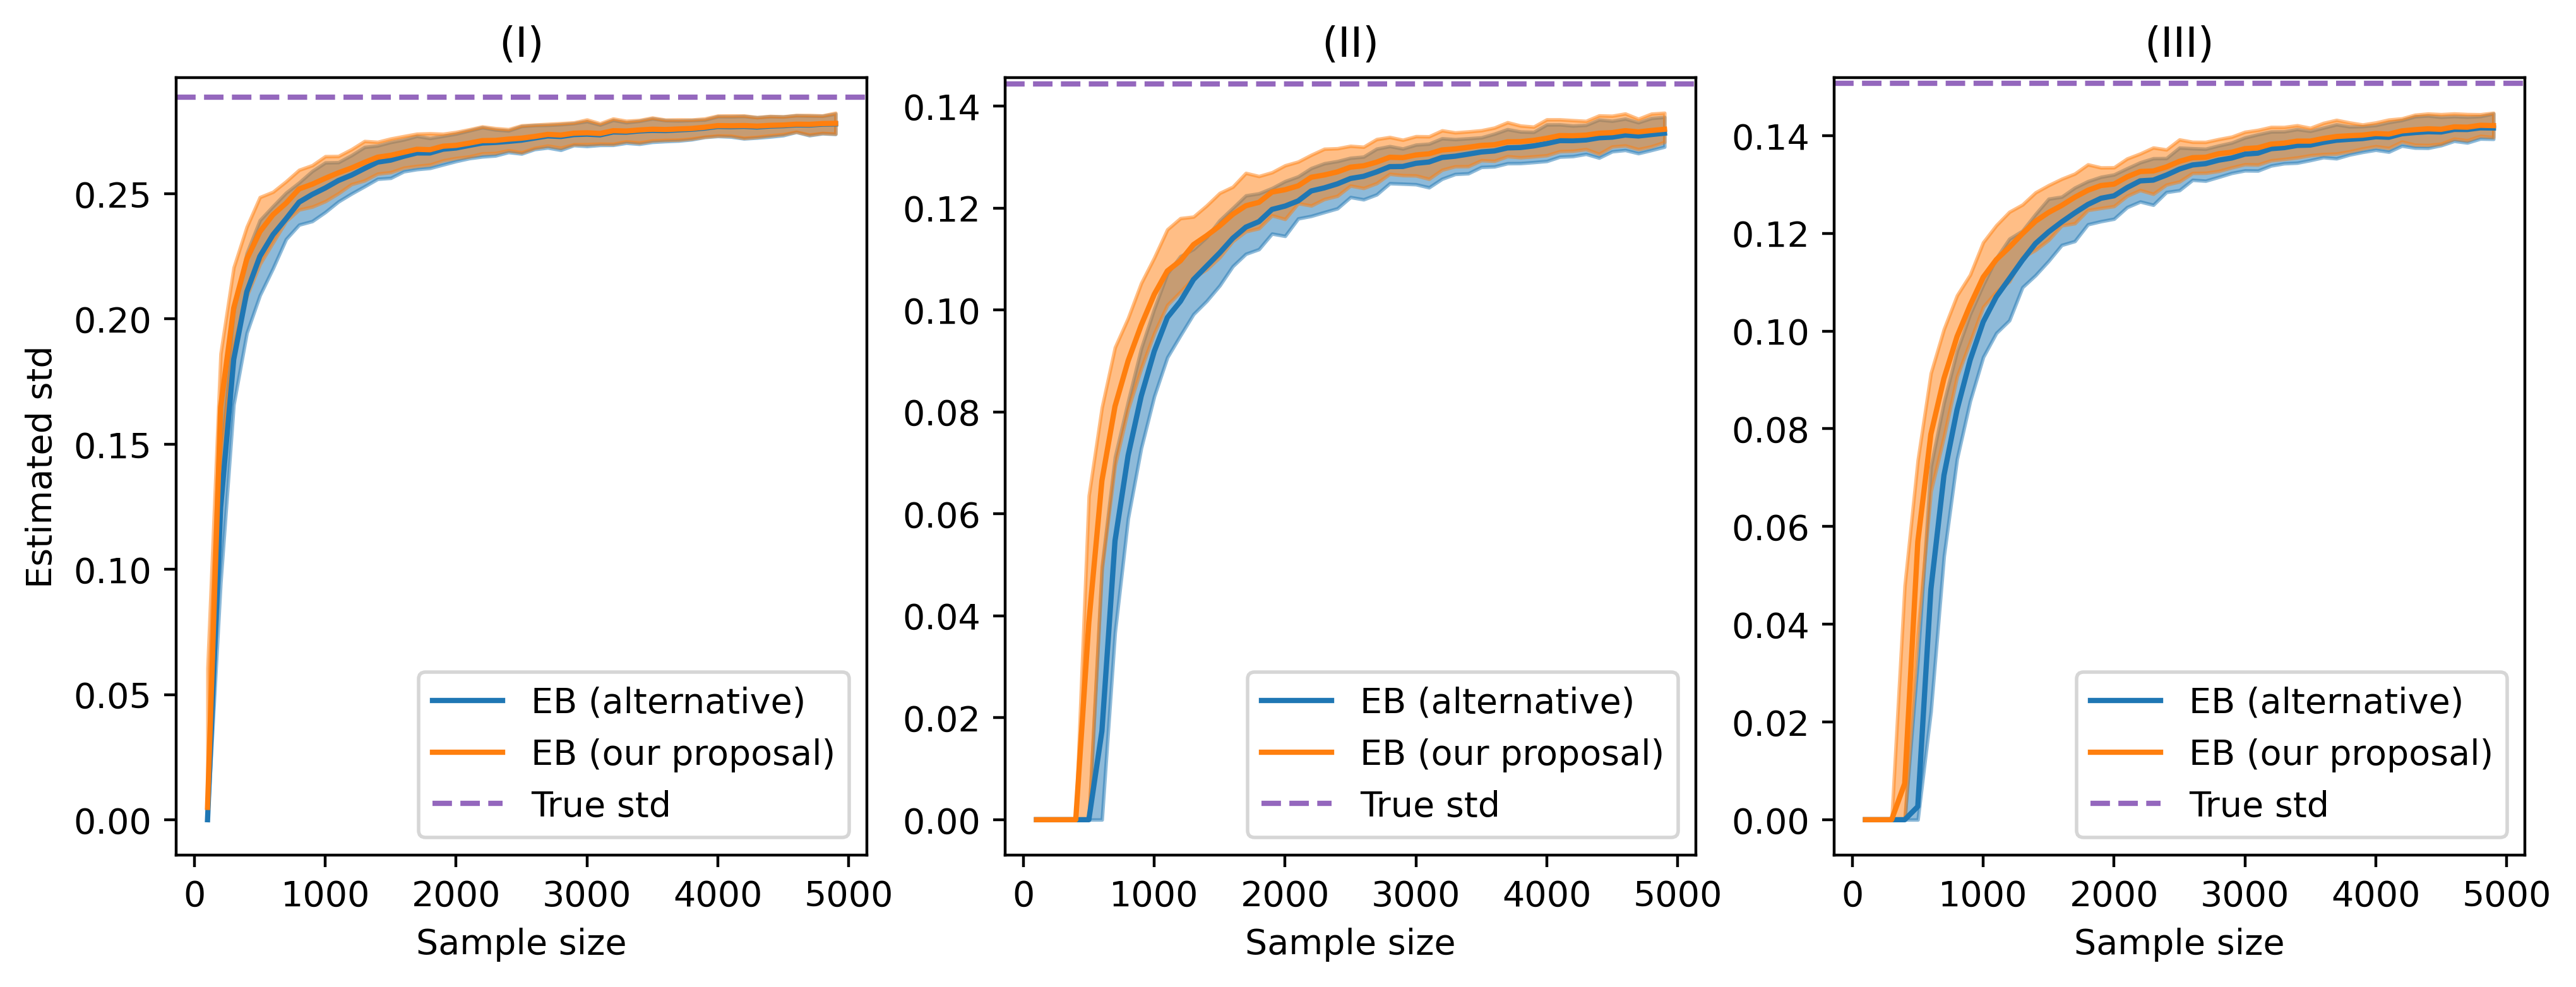
\includegraphics[width=\textwidth]{plots/eb_vs_ebalternative.png}
  \caption{Average confidence intervals over $100$ simulations for the std $\sigma$ for (I) the uniform distribution in $(0,1)$, (II) the beta distribution with parameters $(2, 6)$, and (III) the beta distribution with parameters $(5, 5)$. For each of the inequalities, the $0.95\%$-empirical quantiles are also displayed. The EB lower confidence intervals with the plug-ins from Section~\ref{section:lower_bound} (our proposal) are compared against the EB lower confidence intervals with the plug-ins proposed in this appendix (alternative). Despite the expected similar outcomes, the plug-ins from Section~\ref{section:lower_bound} lead to slightly sharper bounds.} 
  \label{fig:eb_vs_ebalternative}
\end{figure}


\subsection{Known mean}

The main results of this contribution are derived from Corollary~\ref{corollary:main_corollary}. However, Corollary~\ref{corollary:main_corollary} is not readily applicable because $E_t$ is unknown, given that $\mu$ is also unknown in practice. We explore here the power of Corollary~\ref{corollary:main_corollary} in comparison to our final confidence intervals, i.e., how much it is lost after dealing with the unknown term $E_t$. We explore this just as a theoretical exercise, given that $\mu$ is generally unknown. Figure~\ref{fig:known_mu} displays the upper and lower confidence intervals for different sample sizes and distributions. The upper confidence bounds remain essentially unchanged, with the orange and blue regions being nearly indistinguishable. In contrast, the lower bounds exhibit a clear gap, which is consistent with the greater difficulty of deriving lower bounds and the requirement of applying an additional concentration inequality to the empirical mean estimator.

\begin{figure}[!ht] 
    \center 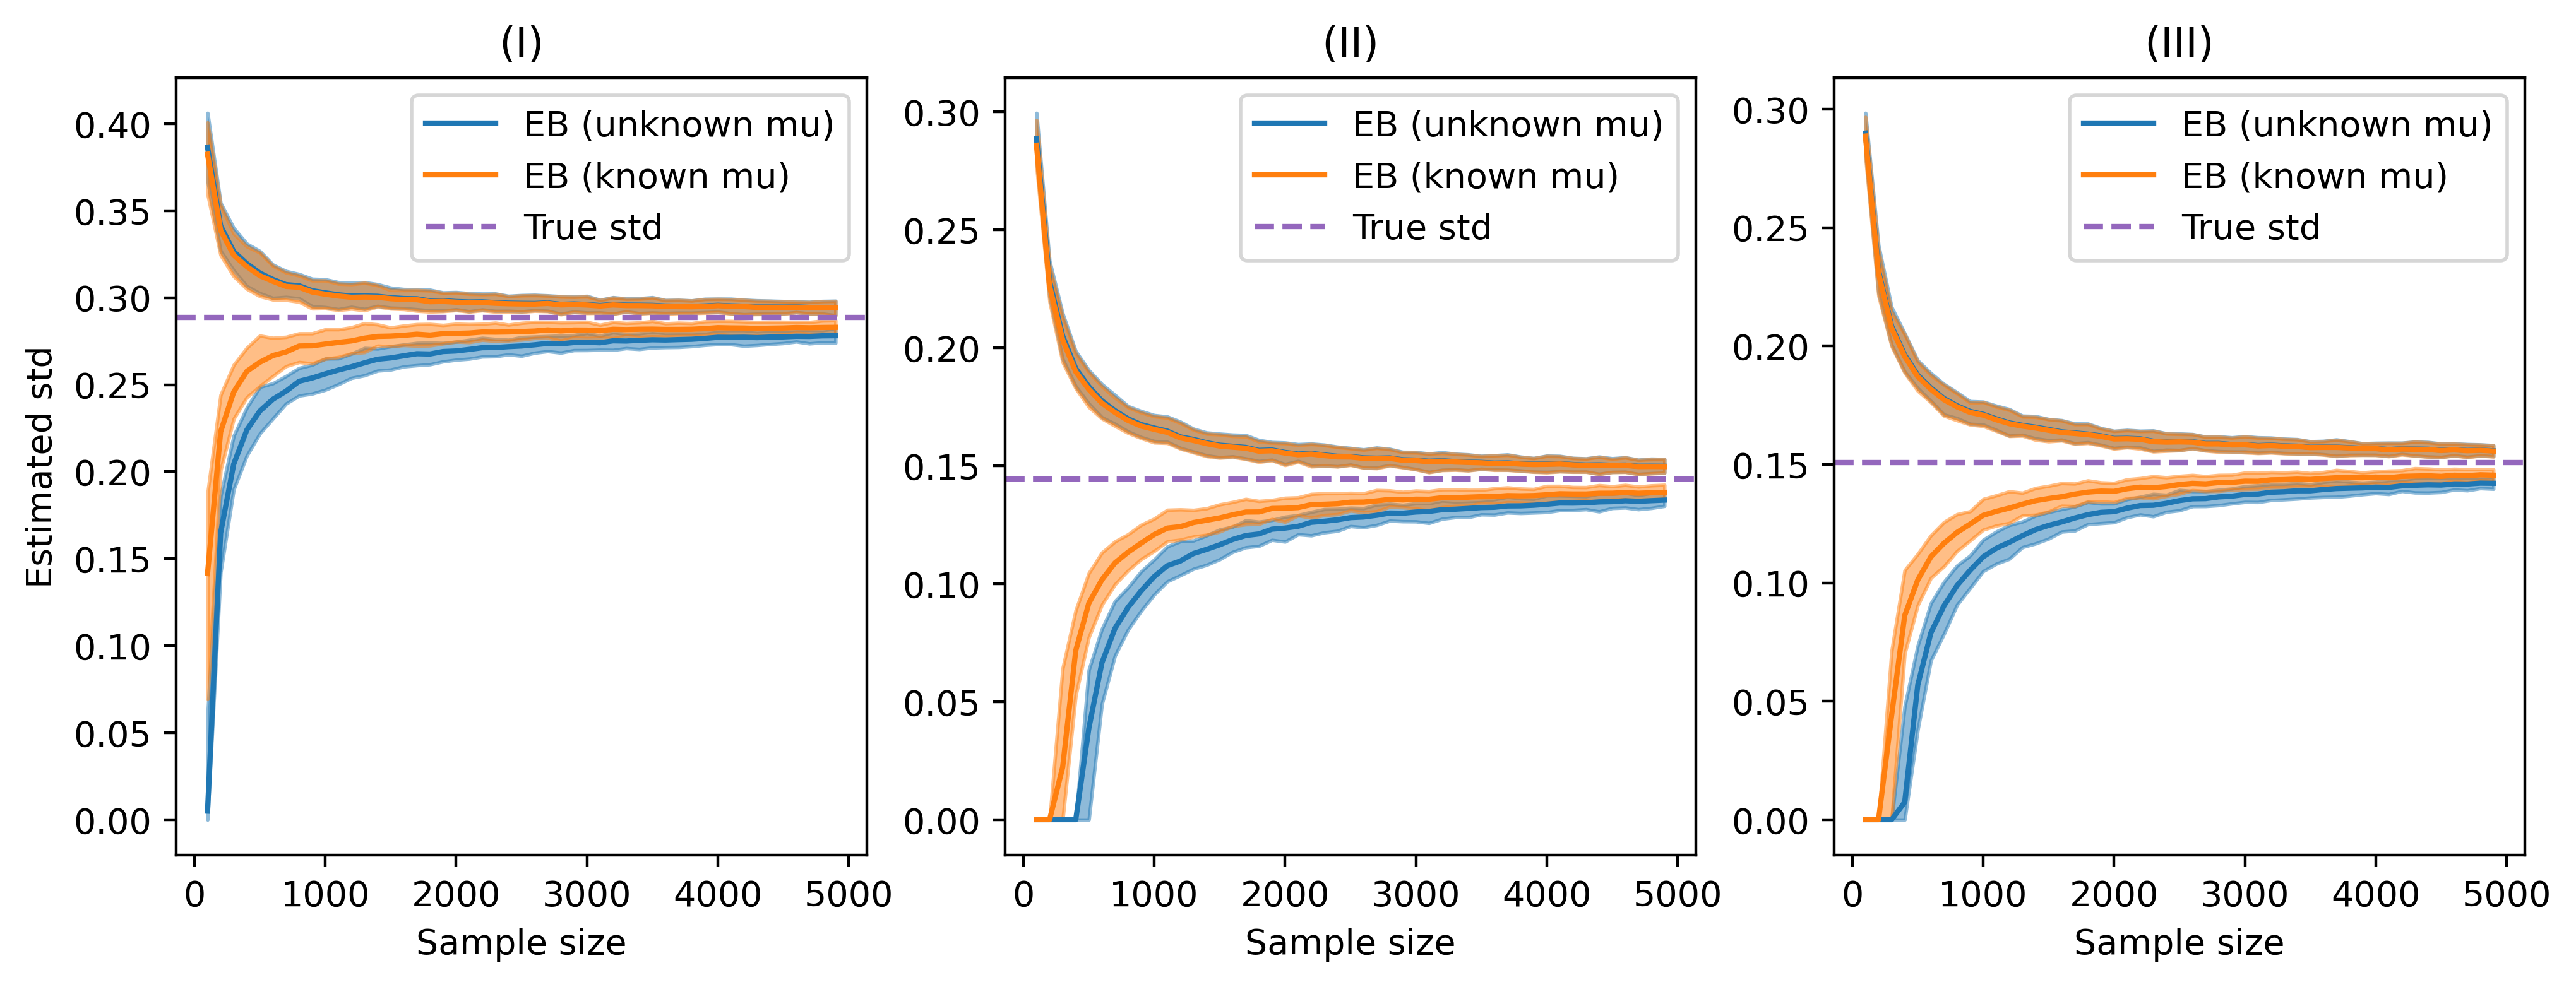
\includegraphics[width=\textwidth]{plots/known_mu.png}
  \caption{Average confidence intervals over $100$ simulations for the std $\sigma$ for (I) the uniform distribution in $(0,1)$, (II) the beta distribution with parameters $(2, 6)$, and (III) the beta distribution with parameters $(5, 5)$. The  confidence intervals proposed in Section~\ref{section:main_results} (EB, unknown mu) are displayed alongside the confidence intervals that could be obtained from Corollary~\ref{corollary:main_corollary} if the mean $\mu$ was known (EB, known mu).} 
  \label{fig:known_mu}
\end{figure}